\subsection{Correlation}

Correlation between the different attributes is not trivial in this case. By plotting the attributes against each other, the majority looks like noise. An exception to this, is the attributes 1 and 7 (not counting \texttt{id}). 

\begin{figure}[H]
\centering
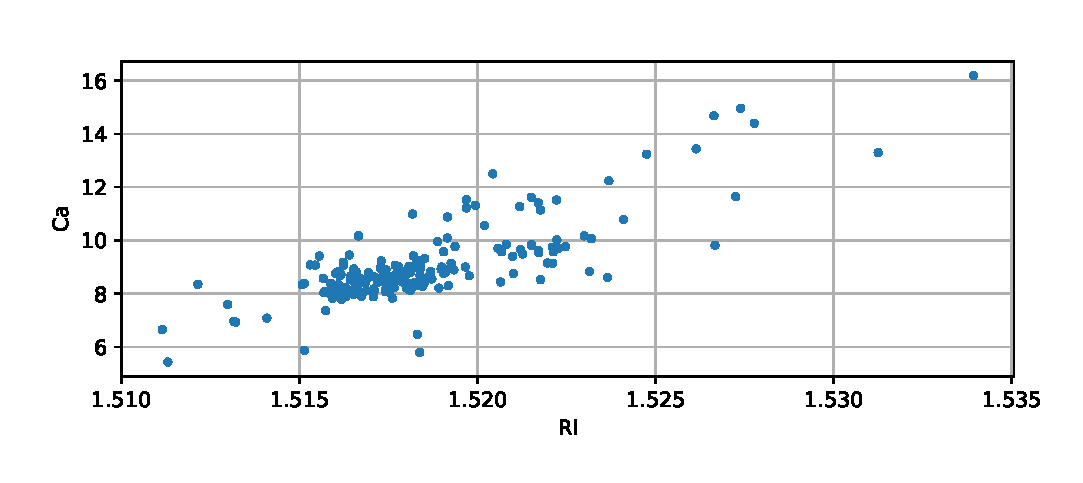
\includegraphics[width=0.9\linewidth]{fig/Correlated.eps} 
\caption{Visualization of attributes 1 (refractive index) and 7 (\texttt{Ca} content), not counting \texttt{id}. Correlation $\approx$ 0.81.  }
\label{fig:correlated}
\end{figure}

As seen in fig \ref{fig:correlated}, these two attributes, refractive index and calcium content, are the most correlated attributes, with a correlation of $\approx$ 0.81. These results visualize what was found in section \ref{sec:CorrMat}.